\newcommand{\authorinfo}{Paul Bienkowski, Hans Ole Hatzel}
\newcommand{\titleinfo}{RS 07 (HA) zum 07.12.2012}

% PREAMBLE ===============================================================

\documentclass[a4paper,10pt]{scrartcl}
\usepackage[german,ngerman]{babel}
\usepackage[utf8]{inputenc}
\usepackage[T1]{fontenc}
\usepackage{lmodern}
\usepackage{amssymb}
\usepackage{mathtools}
\usepackage{amsmath}
\usepackage{enumerate}
\usepackage{array}
\usepackage{listings}
\usepackage{fullpage}
\usepackage[usenames,dvipsnames]{xcolor}
\usepackage{tikz}
\usepackage{circuitikz}
\usepackage{fancyhdr}
\usepackage{lastpage}

\usetikzlibrary{arrows,backgrounds,shapes.gates.logic.US,shapes.gates.logic.IEC,calc,decorations.markings, calc,shapes,arrows}
\usepgfmodule{shapes}

\author{\authorinfo}
\title{\titleinfo}
\date{\today}

\pagestyle{fancy}
\fancyhf{}
\fancyhead[L]{\authorinfo}
\fancyhead[R]{\titleinfo}
\fancyfoot[C]{\thepage}
\renewcommand{\headrulewidth}{0.4pt}
\renewcommand{\footrulewidth}{0pt}
\renewcommand{\headheight}{12pt}
\renewcommand{\headsep}{12pt}

\begin{document}
\setcounter{secnumdepth}{0}
\maketitle

% allow huuuuge matrix
\setcounter{MaxMatrixCols}{31}

% DOCUMENT ===============================================================

\tikzstyle{branch}=[fill,shape=circle,minimum size=3pt,inner sep=0pt]

\newcommand*{\oline}[1]{\overline{\vphantom{A}#1}}

\begin{enumerate}
    \item[\textbf{?.}]
    \begin{enumerate}
        Schaltbild mit 3 Multiplexern:

        \vspace{-2.5cm}
            \includegraphics[angle=-90,width=0.8\textwidth]{mux2-addierer.eps}
        \vspace{-2.5cm}
    \end{enumerate}

\end{enumerate}
\end{document}
